\documentclass{beamer}

% Packages
\usepackage[utf8]{inputenc}
\usepackage{graphicx}
\usepackage{listings} % For code listings
\usepackage{amsmath}
\usepackage{tikz}     % Optional: for custom diagrams

% Document Information
\title{From Traditional Image Processing to Convolutional Neural Networks}
\subtitle{An Introduction to Computer Vision Techniques}
\author{Florian Valade}
\date{\today}

\begin{document}

% Title slide
\begin{frame}
  \titlepage
\end{frame}

% Outline
\begin{frame}{Overview}
  \tableofcontents
\end{frame}

% ------------------------ Section I: Introduction ------------------------
\section{Introduction \& Overview}

\begin{frame}{The Birth of Modern Computer Vision}
  \begin{itemize}
    \item Computer vision has evolved from simple pattern recognition to complex deep learning systems
    \item One of the most significant early breakthroughs: Automated Digit Recognition
    \item Key pioneer: Yann LeCun and his work at Bell Labs (1980s-1990s)
  \end{itemize}
  \begin{center}
    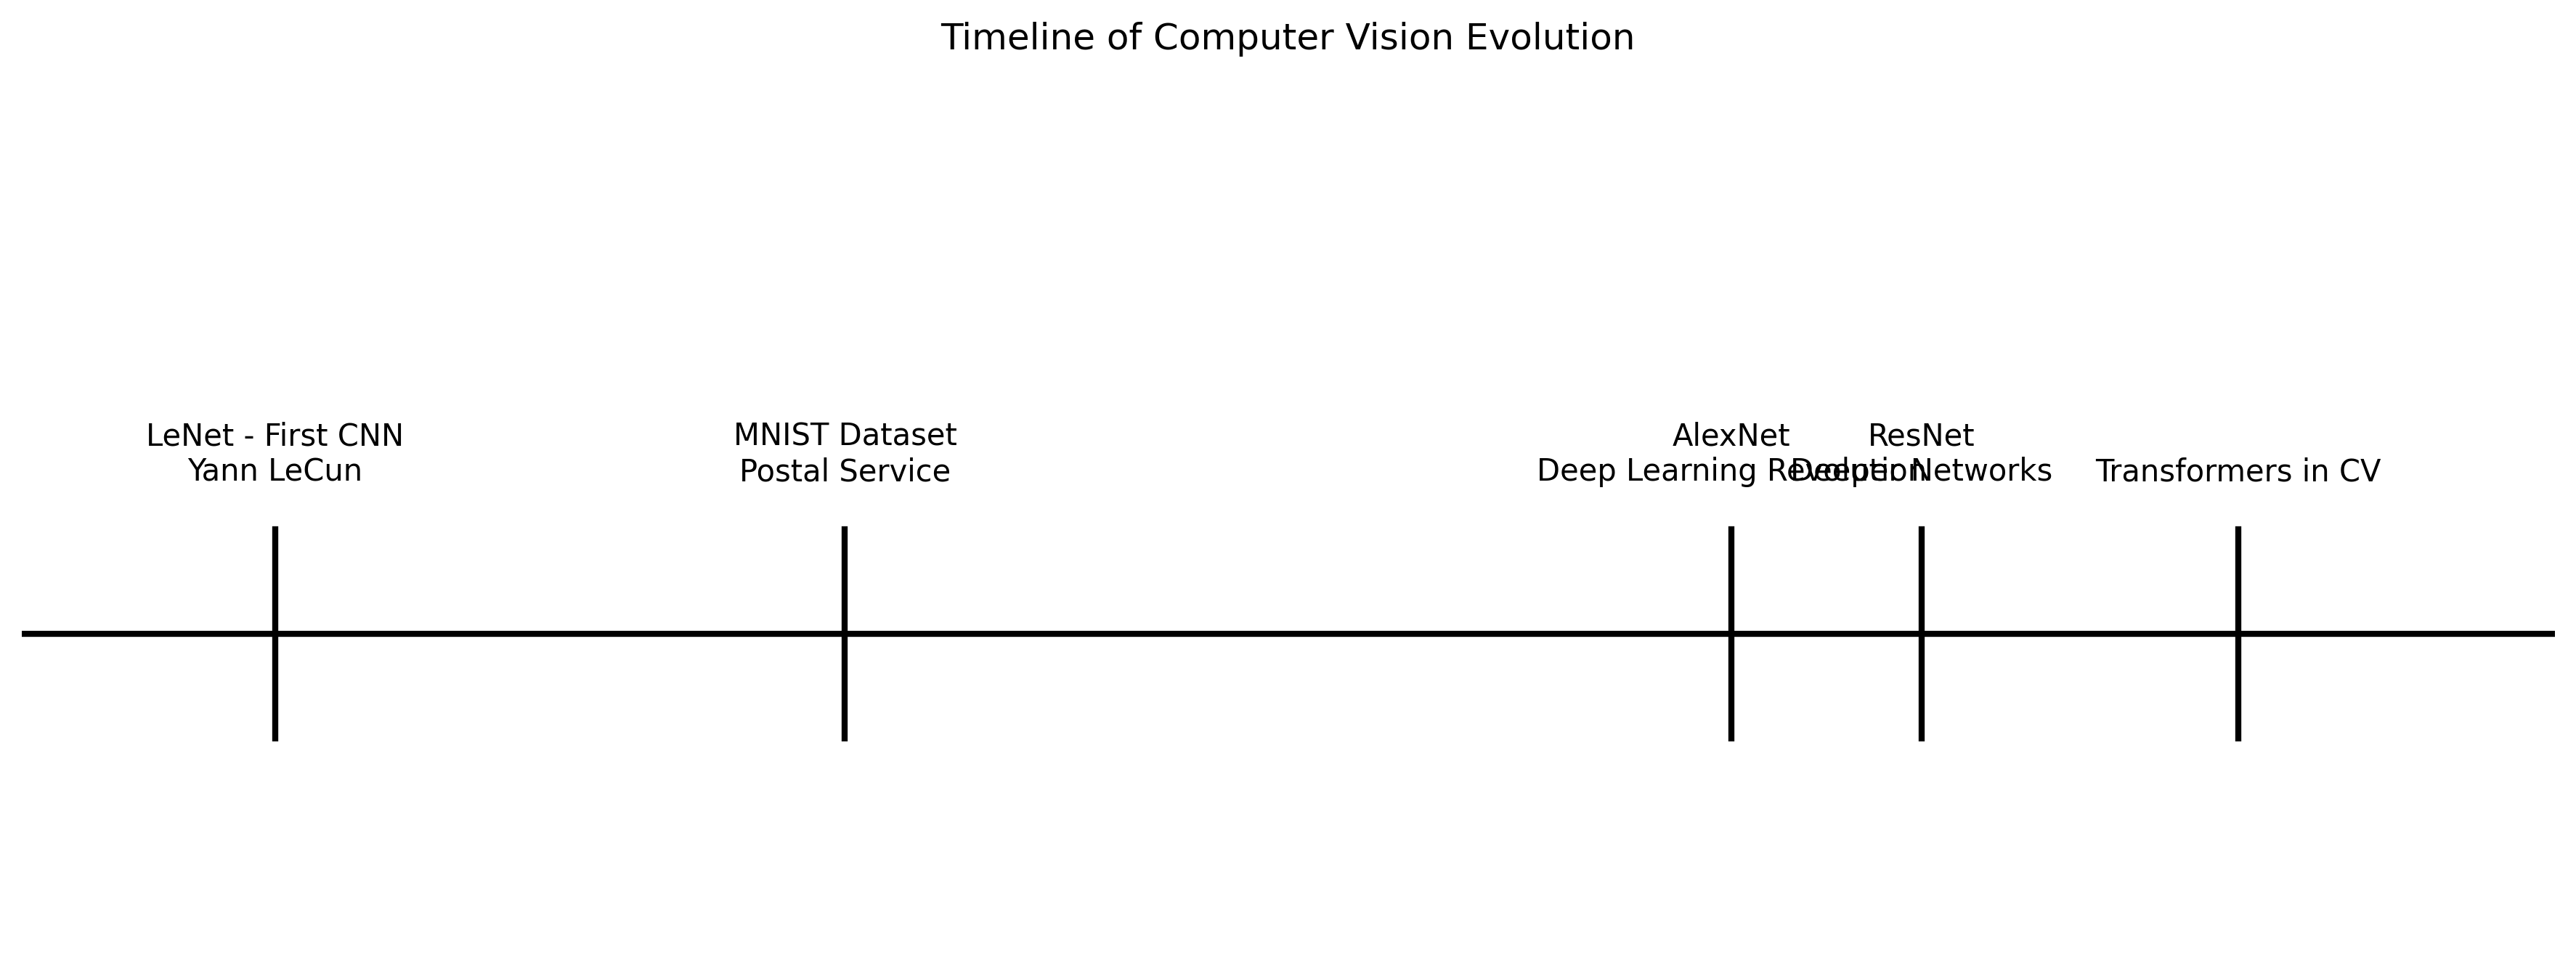
\includegraphics[width=0.8\textwidth]{images/timeline_cv.png}
  \end{center}
\end{frame}

\begin{frame}{The First Major Application: Postal Service}
  \begin{itemize}
    \item First large-scale real-world application: Automated ZIP code reading
    \item Deployed by the U.S. Postal Service in the late 1990s
    \item Processed millions of pieces of mail daily
  \end{itemize}
  \begin{center}
    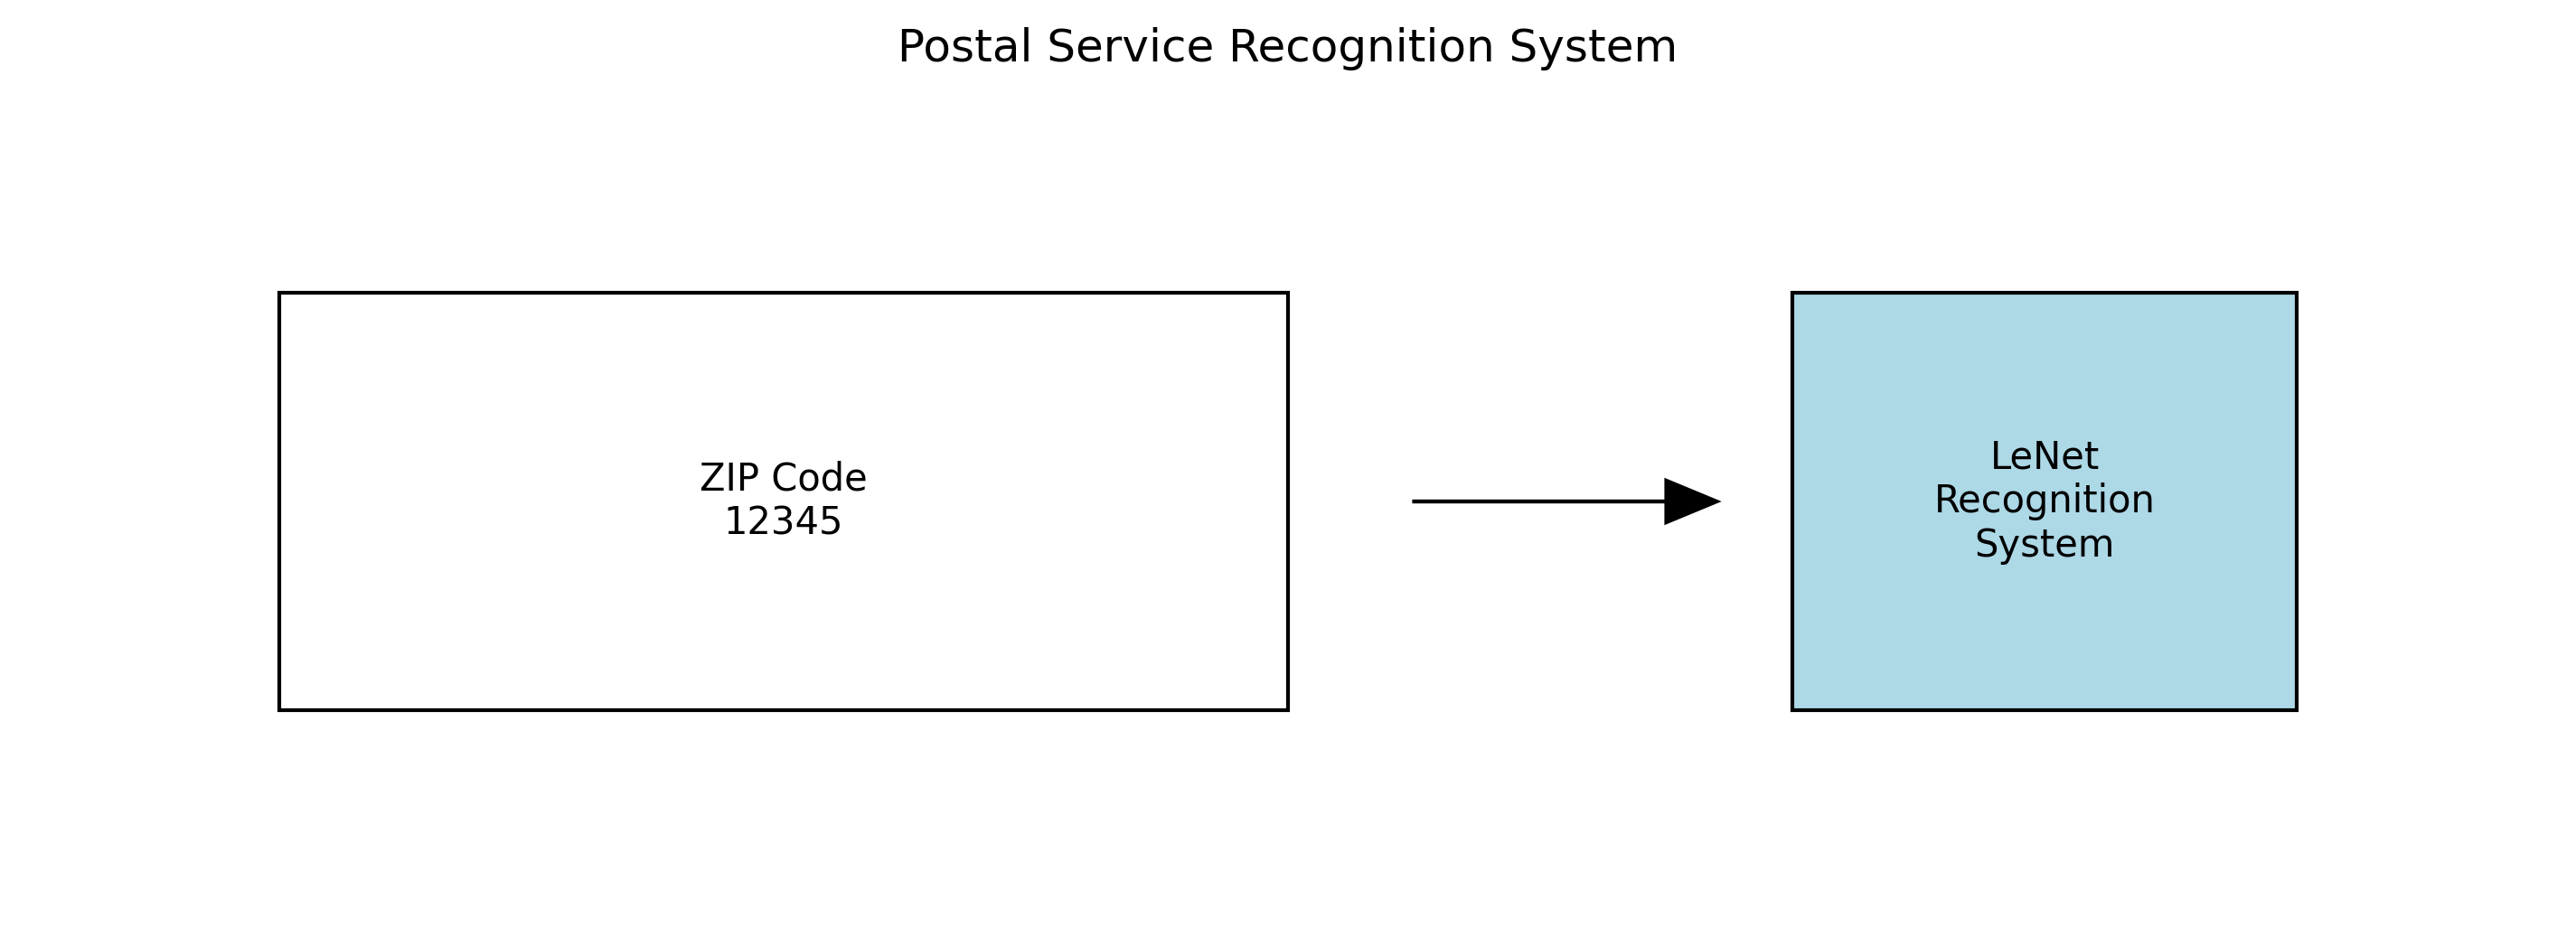
\includegraphics[width=0.9\textwidth]{images/postal_recognition.png}
  \end{center}
\end{frame}

\begin{frame}{The MNIST Dataset}
  \begin{itemize}
    \item Created from the National Institute of Standards and Technology (NIST) database
    \item Modified and normalized by Yann LeCun's team
    \item Became the "Hello World" of machine learning
    \item 60,000 training images, 10,000 test images
  \end{itemize}
  \begin{center}
    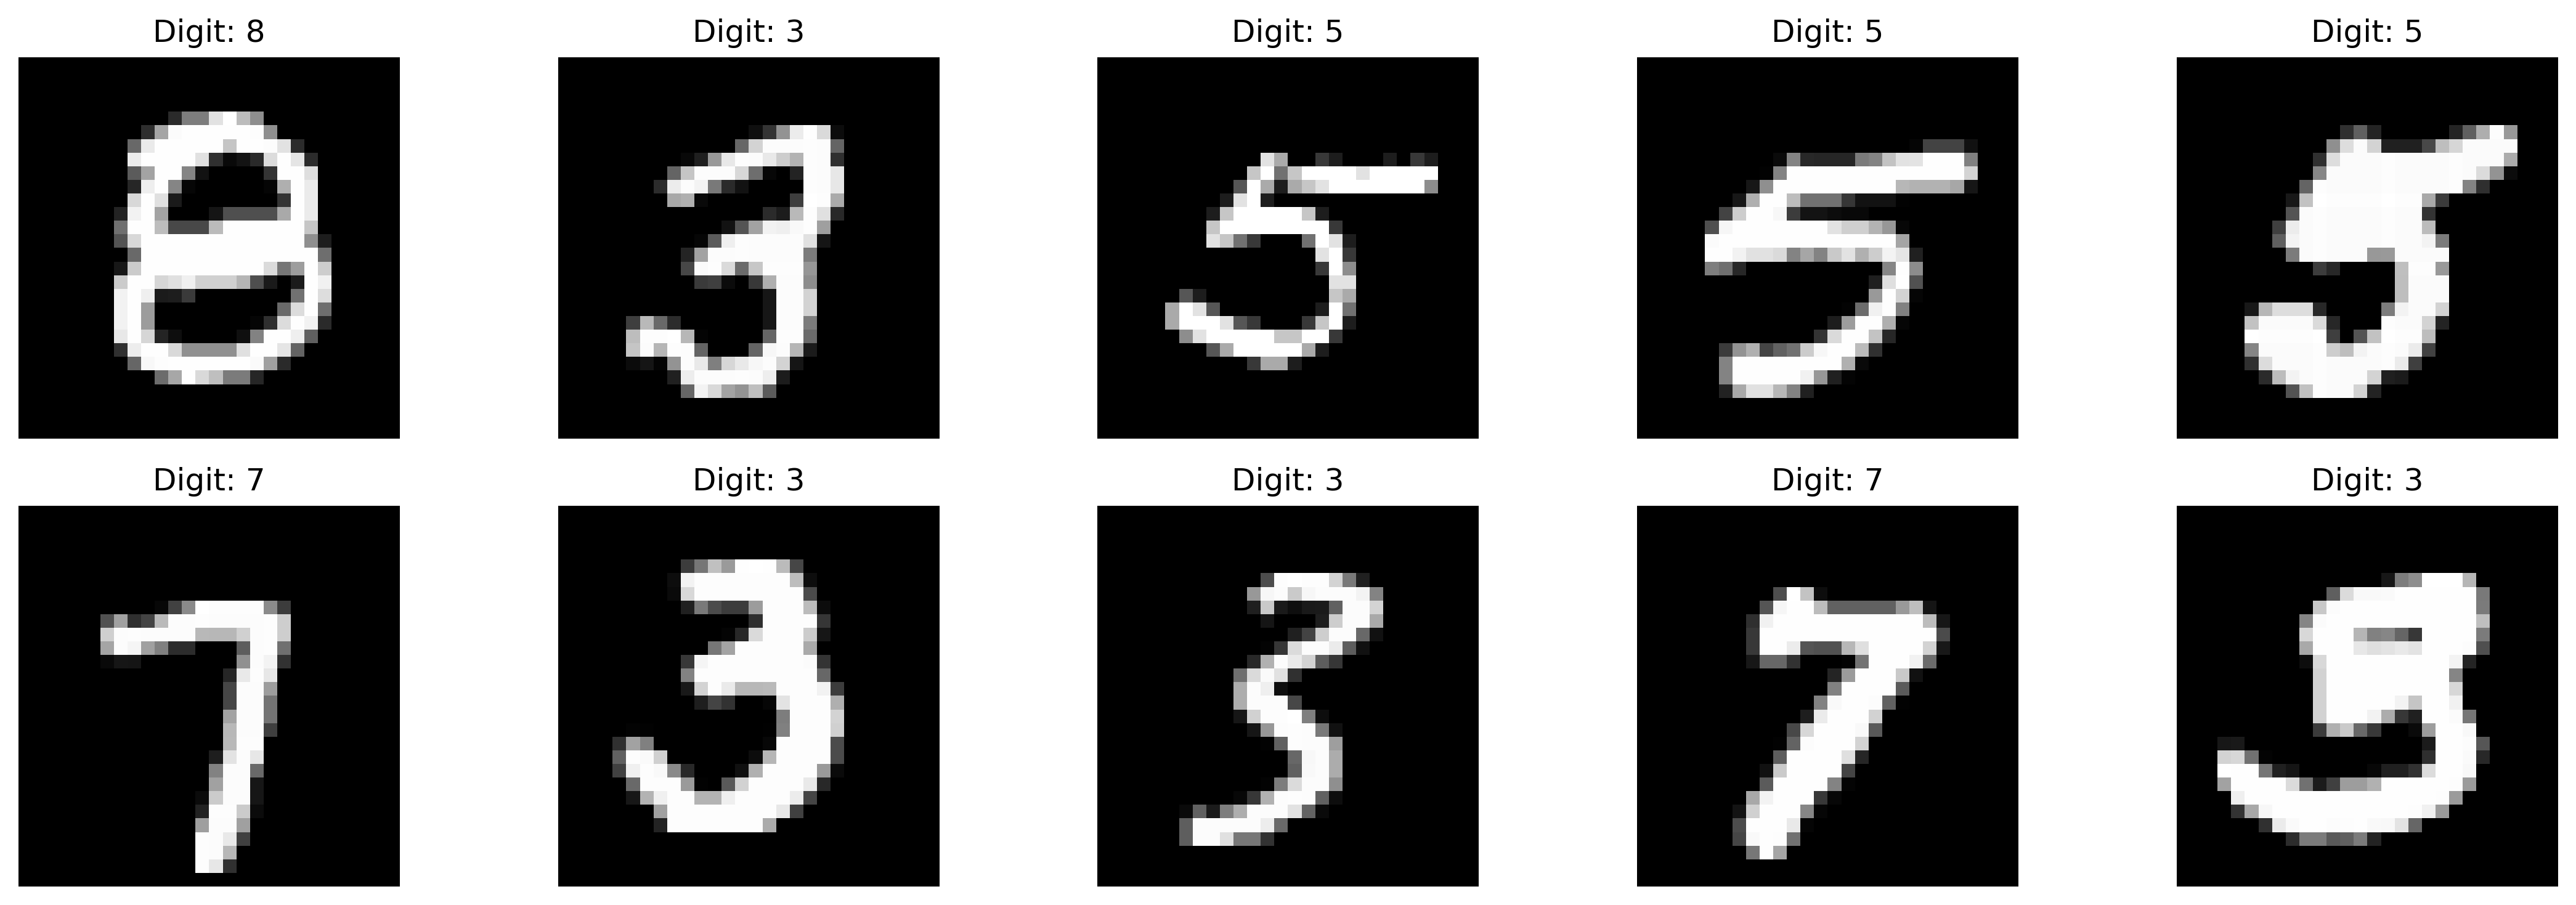
\includegraphics[width=0.8\textwidth]{images/mnist_samples.png}
  \end{center}
\end{frame}

\begin{frame}{LeNet-5: The Pioneer Architecture}
  \begin{itemize}
    \item First successful Convolutional Neural Network (CNN)
    \item Key innovations:
      \begin{itemize}
        \item Local receptive fields
        \item Shared weights
        \item Subsampling layers
      \end{itemize}
    \item Achieved 99.2\% accuracy on digit recognition
  \end{itemize}
  \begin{center}
    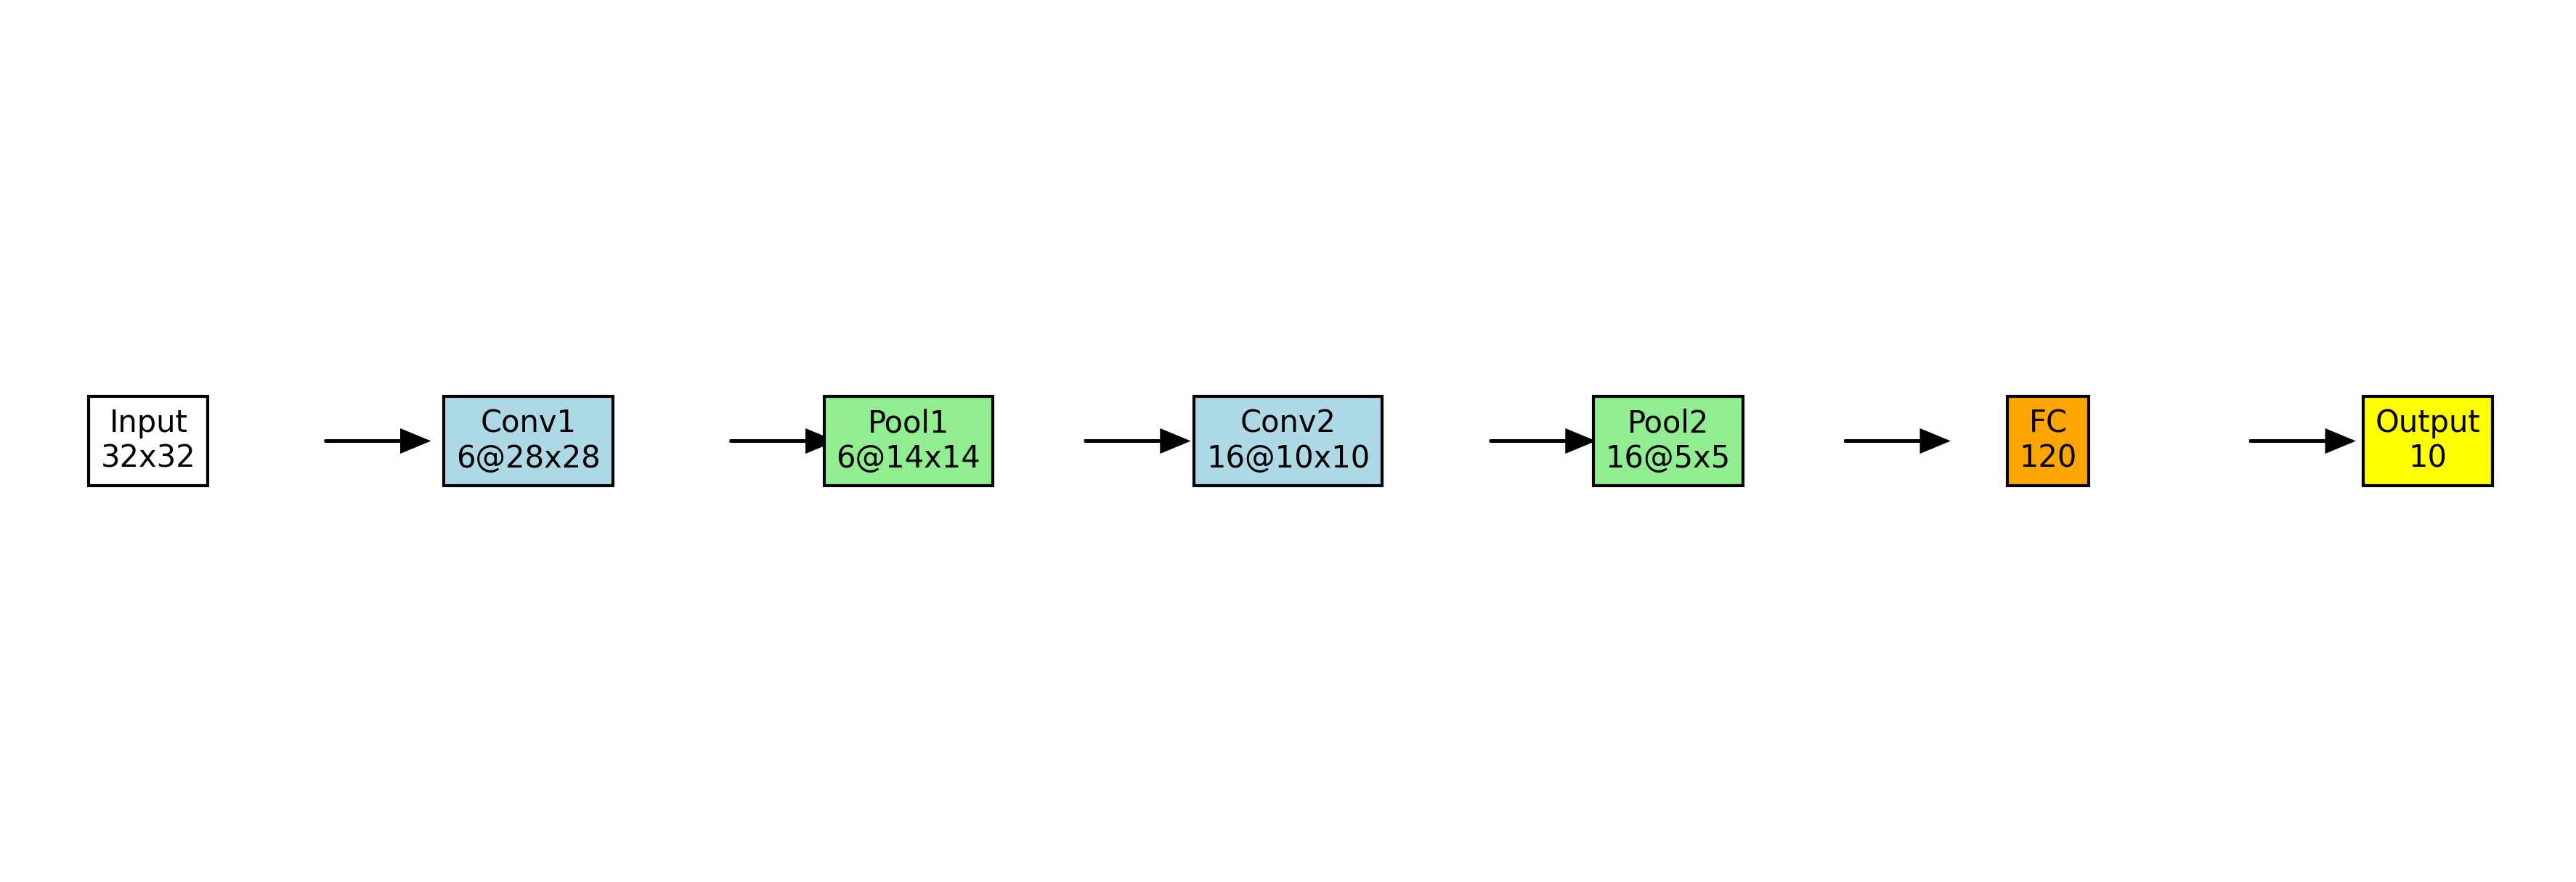
\includegraphics[width=0.9\textwidth]{images/lenet.png}
  \end{center}
\end{frame}

\begin{frame}{Impact and Legacy}
  \begin{itemize}
    \item LeNet's architecture became the foundation for modern CNNs
    \item Key principles still used in state-of-the-art networks:
      \begin{itemize}
        \item Convolutional layers for feature extraction
        \item Pooling layers for dimensionality reduction
        \item Dense layers for final classification
      \end{itemize}
    \item Demonstrated the potential of deep learning for real-world applications
  \end{itemize}
\end{frame}

% ------------------------ Section II: Traditional Image Processing ------------------------
\section{Understanding Digital Images}

\begin{frame}{What is a Digital Image?}
  \begin{itemize}
    \item A digital image is a 2D grid of pixels (picture elements)
    \item Each pixel represents:
      \begin{itemize}
        \item A single intensity value (grayscale images)
        \item Multiple color channel values (RGB images)
      \end{itemize}
    \item Pixel values typically range from 0 (black) to 255 (white)
  \end{itemize}
  \begin{center}
    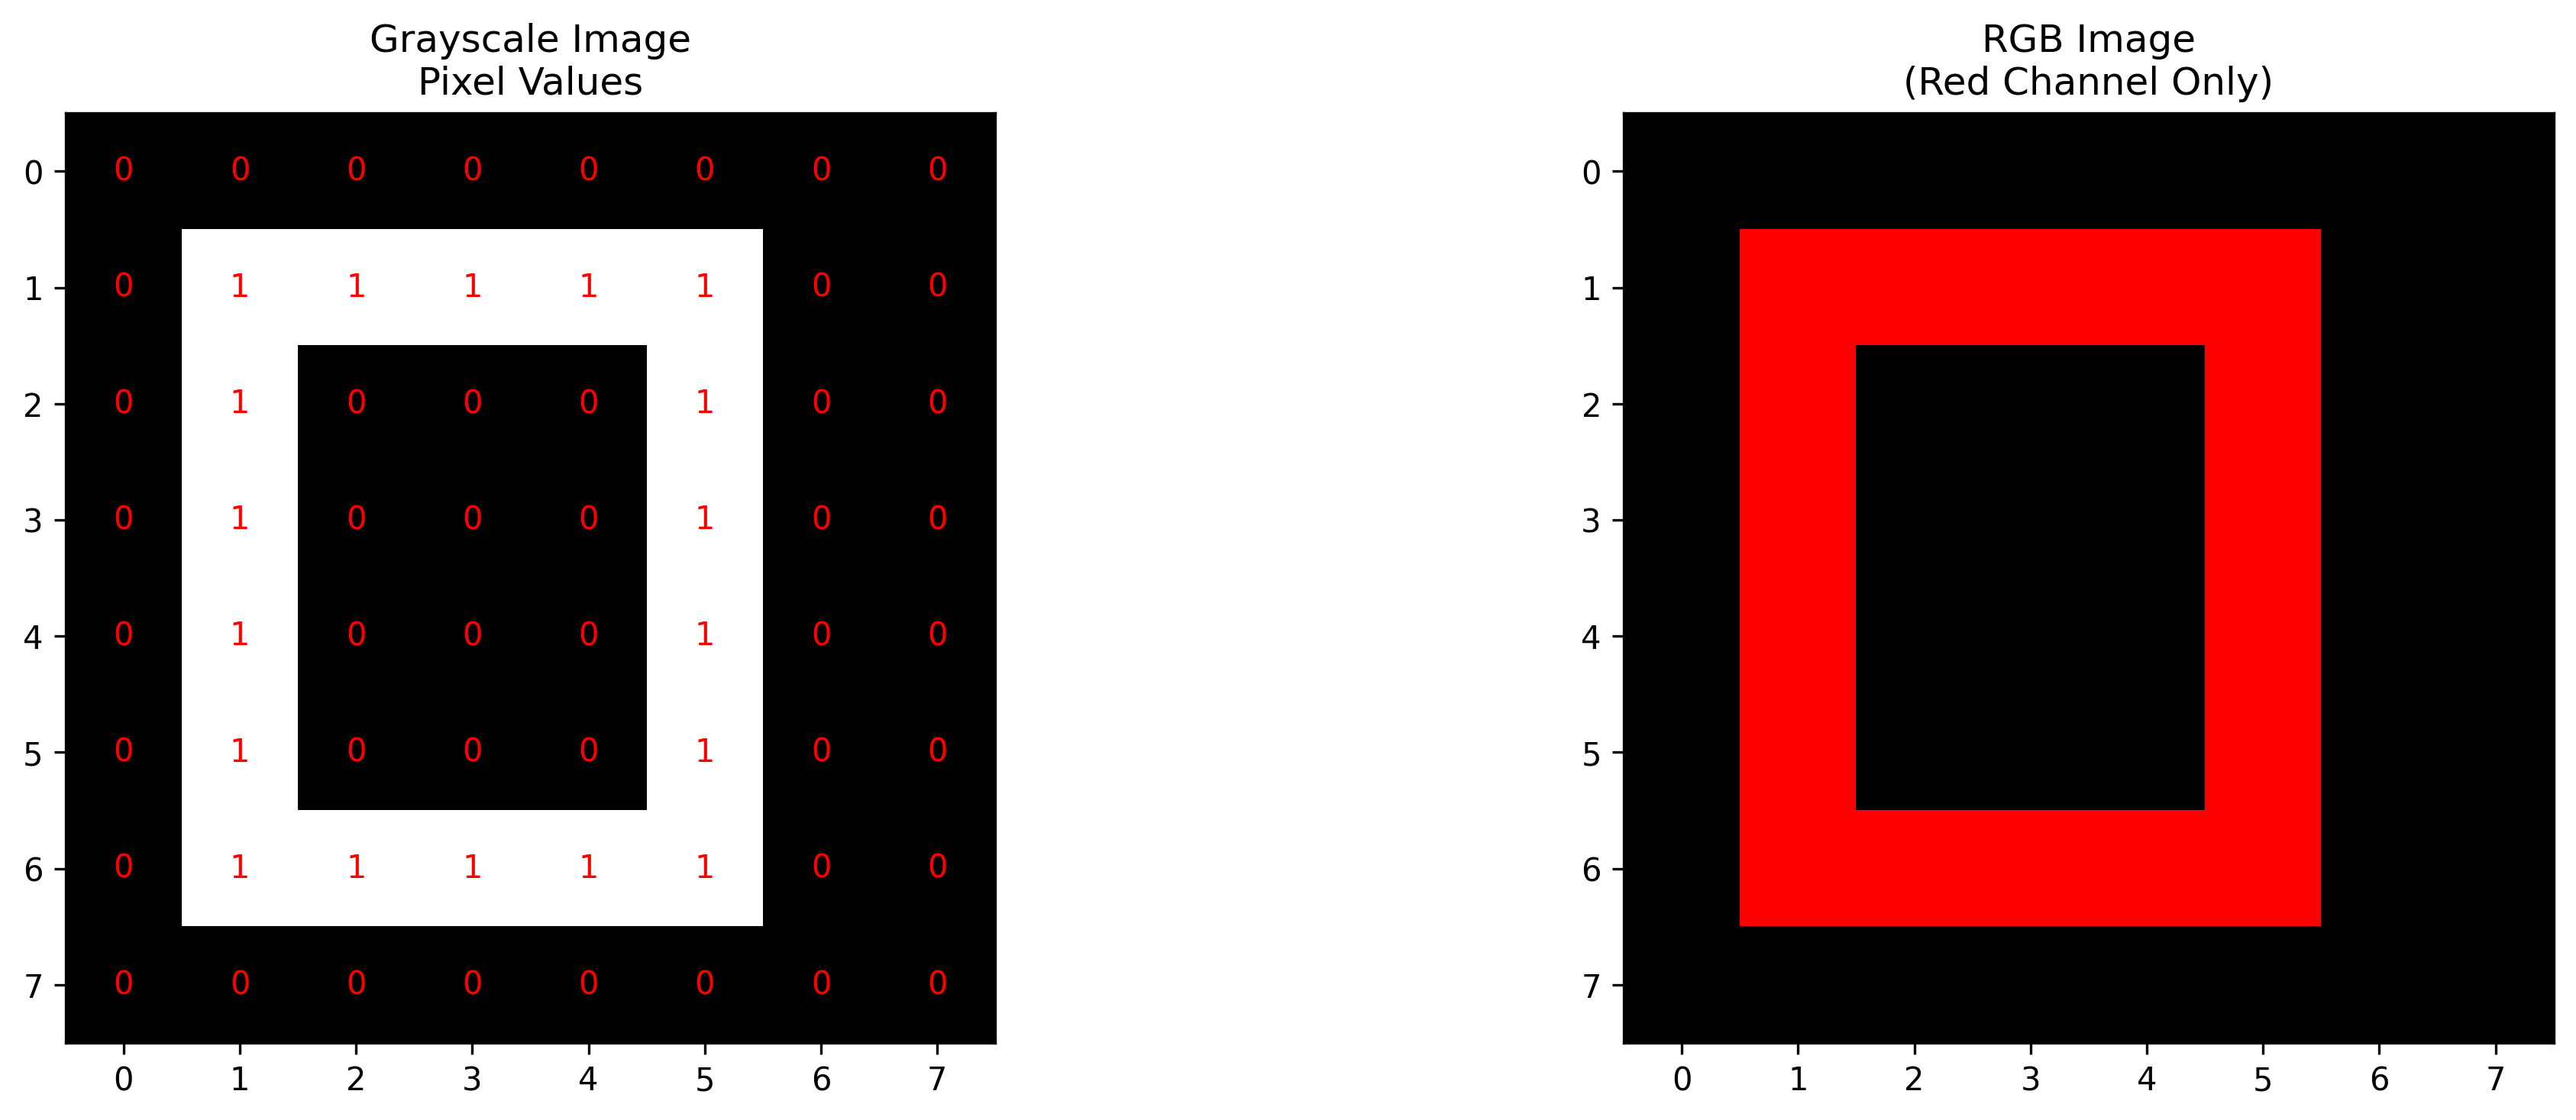
\includegraphics[width=0.9\textwidth]{images/image_representation.png}
  \end{center}
\end{frame}

\begin{frame}{Image Types and Color Spaces}
  \begin{columns}
    \column{0.5\textwidth}
      \textbf{Grayscale Images:}
      \begin{itemize}
        \item Single channel
        \item Values: [0, 255]
        \item Used for: Edge detection, texture analysis
      \end{itemize}
    \column{0.5\textwidth}
      \textbf{RGB Images:}
      \begin{itemize}
        \item 3 channels (Red, Green, Blue)
        \item Each channel: [0, 255]
        \item 16.7 million possible colors
      \end{itemize}
  \end{columns}
  \begin{itemize}
    \item Other color spaces: HSV (Hue, Saturation, Value), LAB, YCbCr
    \item Choice depends on application (e.g., HSV for color-based segmentation)
  \end{itemize}
\end{frame}

\begin{frame}{Introduction to Convolution}
  \begin{itemize}
    \item Convolution is the fundamental operation in image processing
    \item It involves:
      \begin{itemize}
        \item A kernel (filter) - small matrix of weights
        \item Sliding this kernel over the image
        \item Computing weighted sums at each position
      \end{itemize}
  \end{itemize}
  \begin{center}
    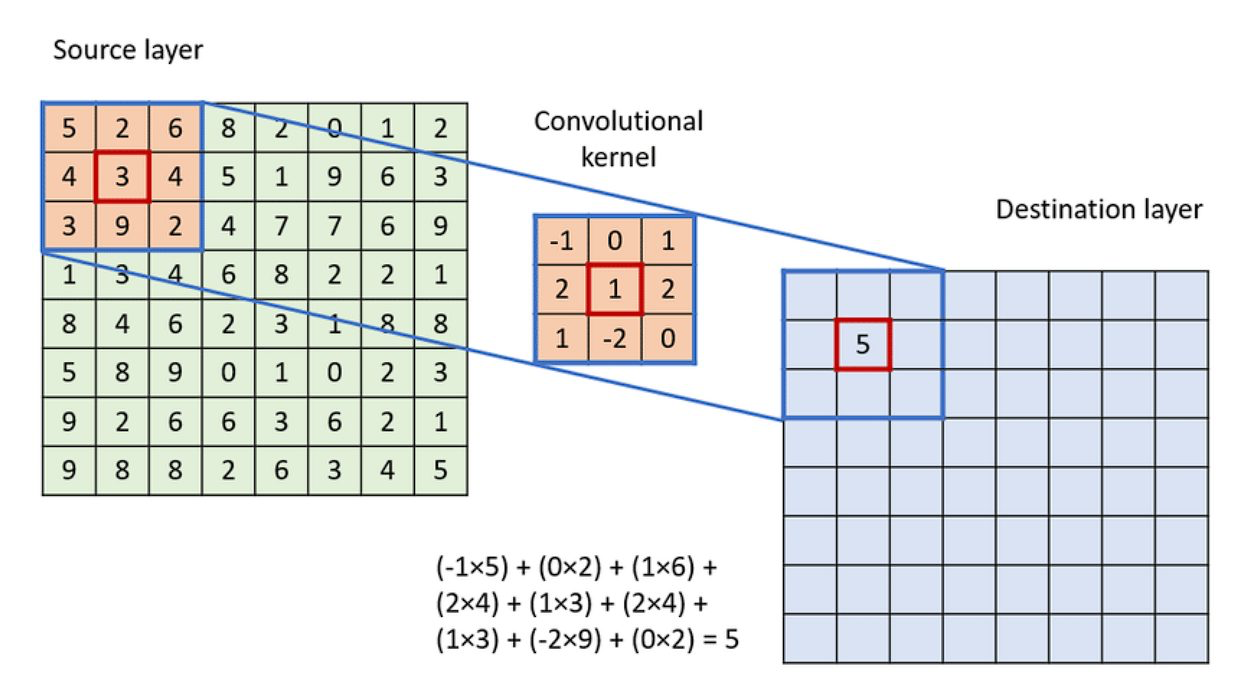
\includegraphics[width=0.9\textwidth]{images/conv_detail.png}
  \end{center}
\end{frame}

\begin{frame}{Understanding Convolution Step by Step}
  \begin{itemize}
    \item Example with a simple mean filter (averaging)
    \item Each output pixel is the average of its 3x3 neighborhood
    \item Helps understand how CNNs process images
  \end{itemize}
  \begin{center}
    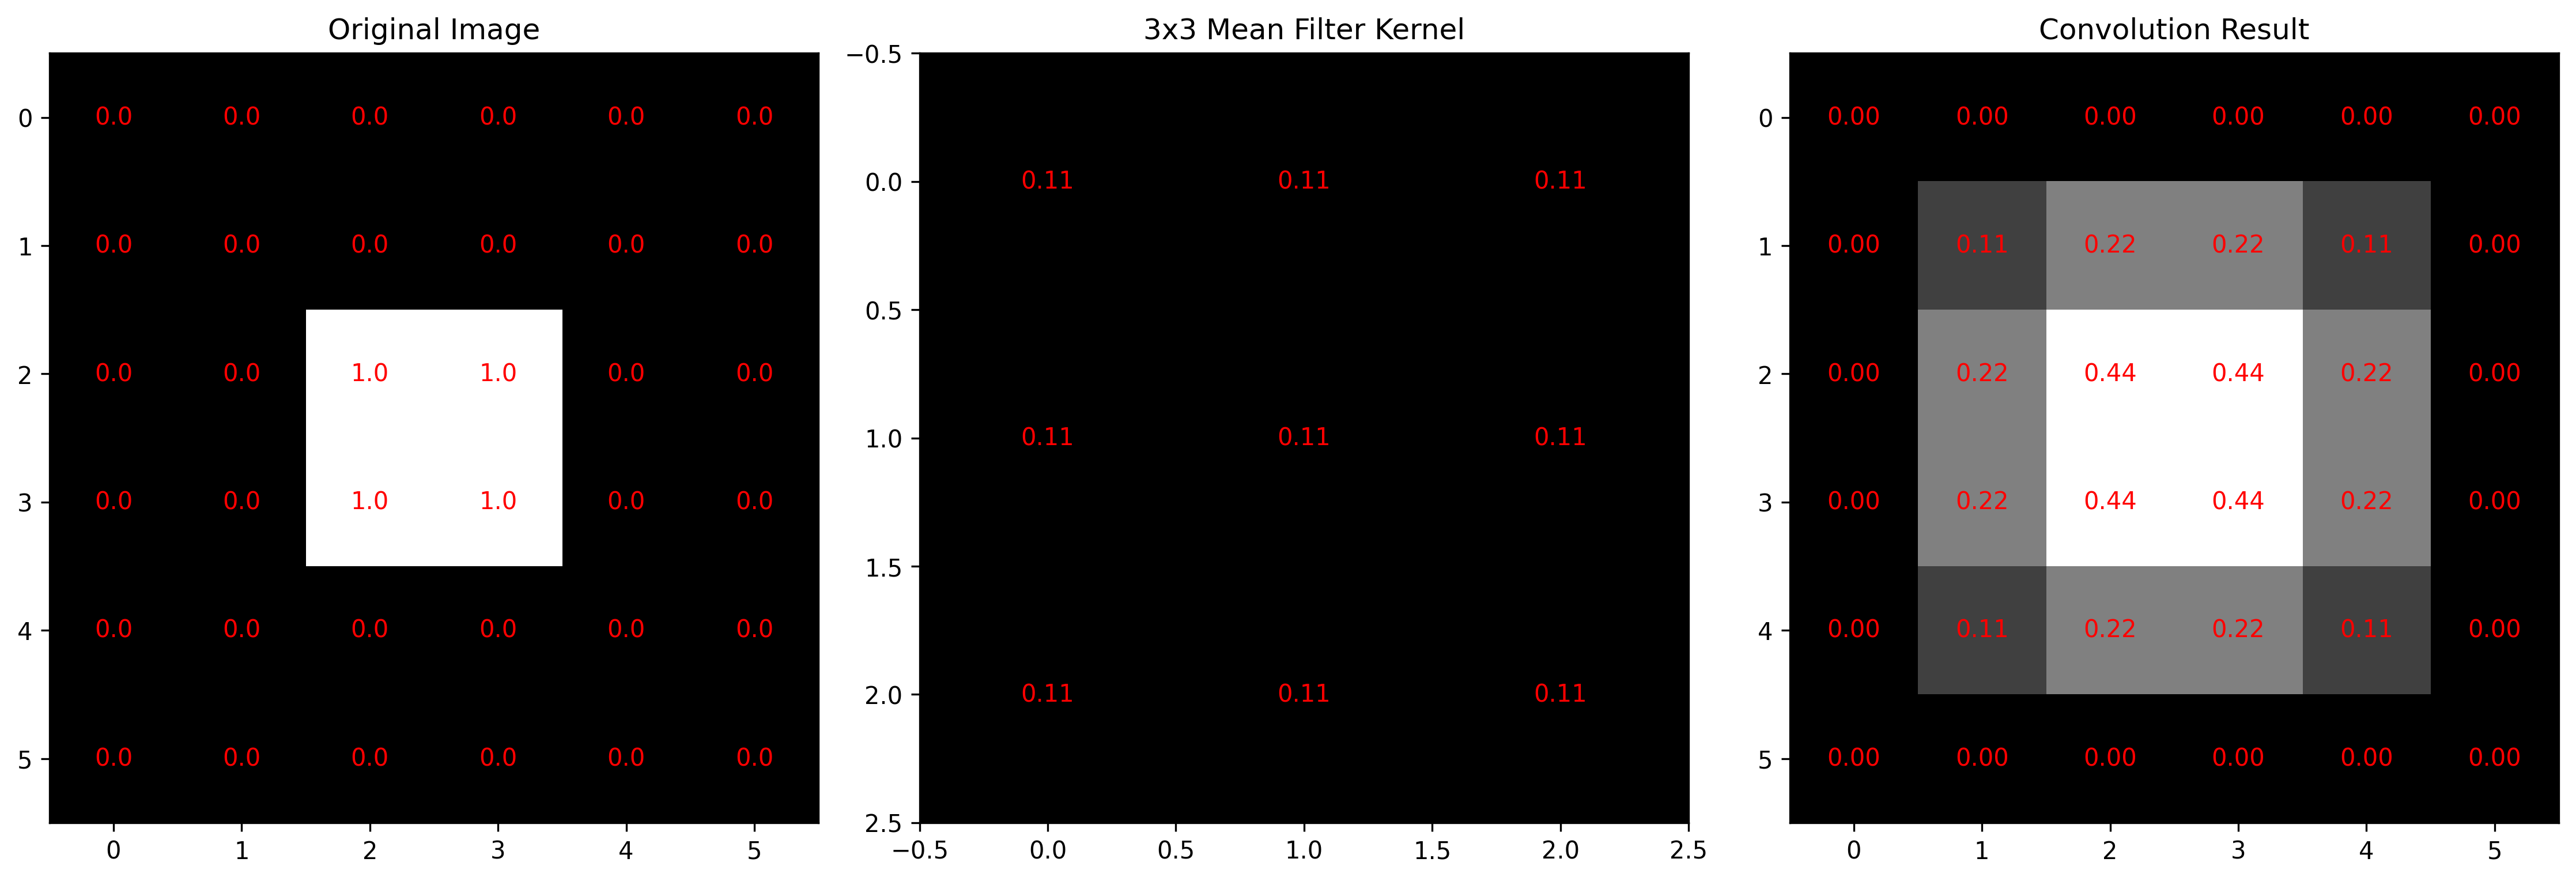
\includegraphics[width=0.9\textwidth]{images/convolution_basic.png}
  \end{center}
\end{frame}

\begin{frame}{Different Types of Kernels}
  \begin{itemize}
    \item Different kernels produce different effects:
      \begin{itemize}
        \item Mean Filter: Smoothing/Blurring
        \item Gaussian Filter: Weighted smoothing
        \item Edge Detection: Highlighting boundaries
      \end{itemize}
  \end{itemize}
  \begin{center}
    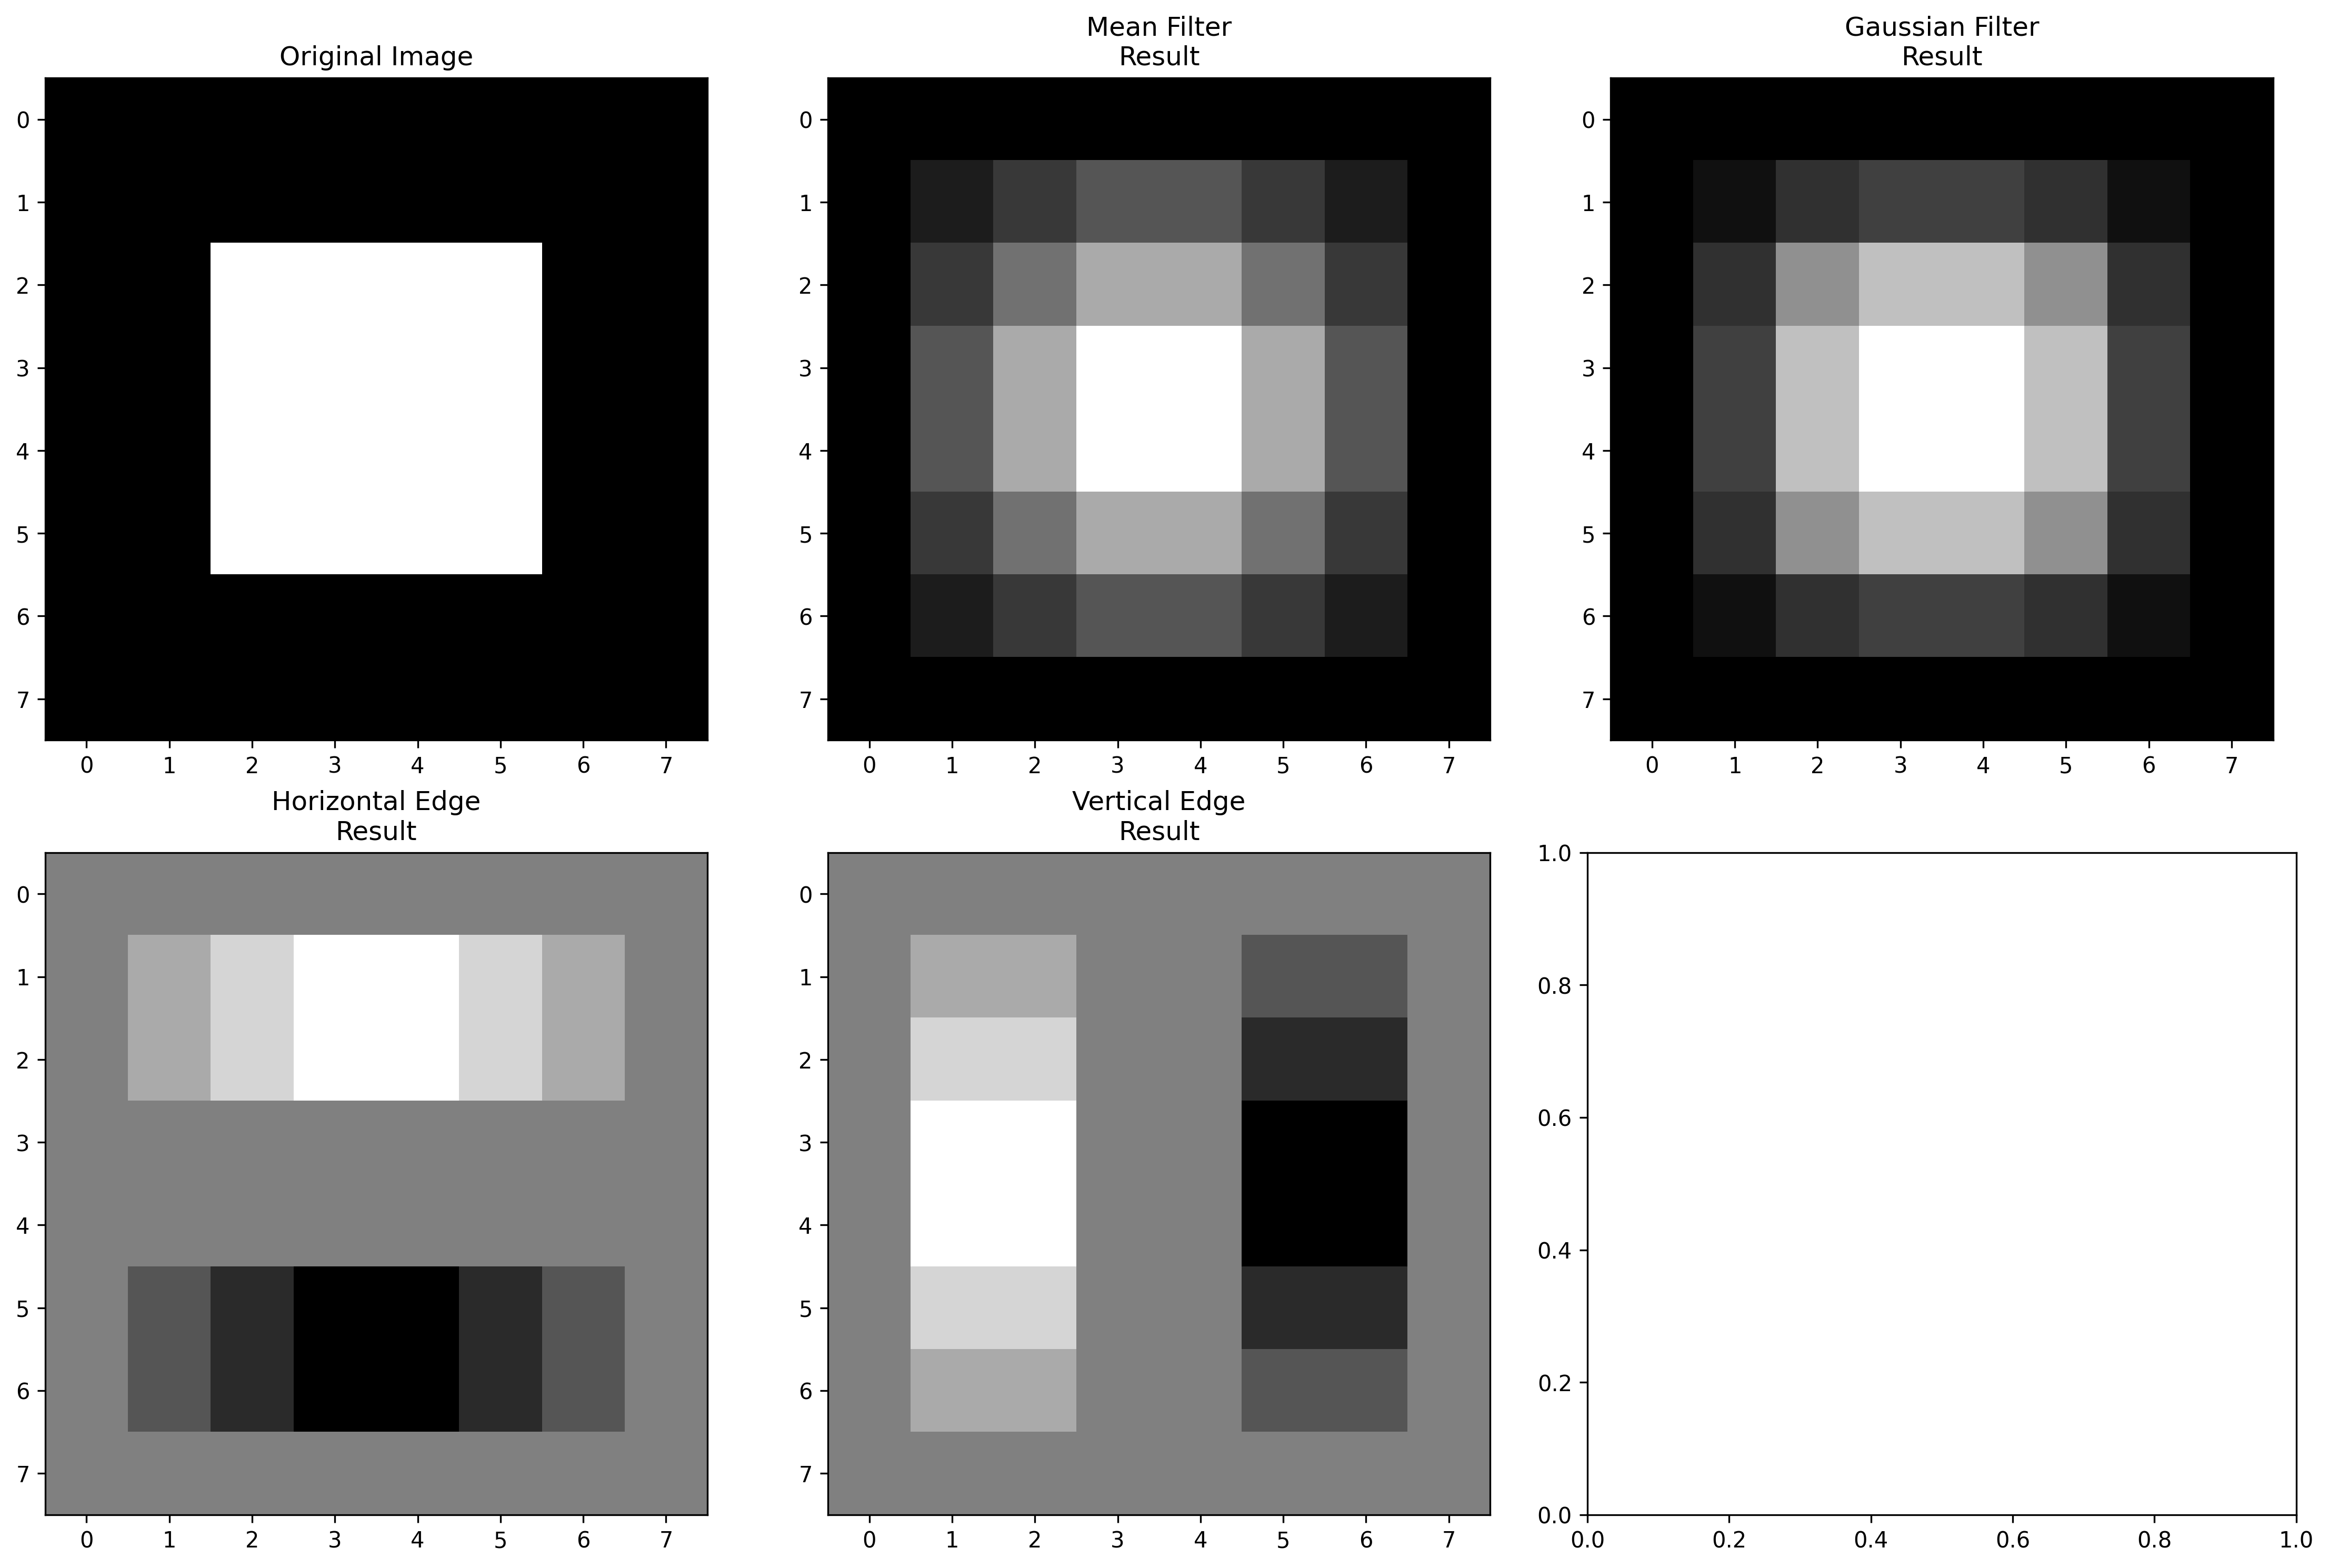
\includegraphics[width=0.9\textwidth]{images/different_kernels.png}
  \end{center}
\end{frame}

\begin{frame}{Mathematical Expression of Convolution}
  For a 2D image \(f\) and a kernel \(g\), convolution is defined as:
  \[
    (f * g)(x,y) = \sum_{i=-k}^{k} \sum_{j=-k}^{k} f(x-i, y-j) \cdot g(i,j)
  \]
  where:
  \begin{itemize}
    \item \((x,y)\) is the position in the output image
    \item \(k\) is the kernel size (typically 1 for 3x3 kernels)
    \item \(f(x-i, y-j)\) is the input pixel value
    \item \(g(i,j)\) is the kernel weight
  \end{itemize}
\end{frame}

\begin{frame}{Properties of Convolution}
  \begin{itemize}
    \item \textbf{Linearity:}
      \begin{itemize}
        \item \(f * (g_1 + g_2) = (f * g_1) + (f * g_2)\)
        \item \(f * (ag) = a(f * g)\)
      \end{itemize}
    \item \textbf{Shift Invariance:}
      \begin{itemize}
        \item Same operation applied at every position
        \item Key property for pattern recognition
      \end{itemize}
    \item \textbf{Boundary Handling:}
      \begin{itemize}
        \item Padding strategies: zero, reflect, replicate
        \item Affects output size and border behavior
      \end{itemize}
  \end{itemize}
\end{frame}

\begin{frame}{Practical Considerations}
  \begin{itemize}
    \item \textbf{Kernel Size:}
      \begin{itemize}
        \item Larger kernels = more context, but slower
        \item Common sizes: 3x3, 5x5, 7x7
      \end{itemize}
    \item \textbf{Normalization:}
      \begin{itemize}
        \item Sum of kernel weights often = 1
        \item Preserves image brightness
      \end{itemize}
    \item \textbf{Separability:}
      \begin{itemize}
        \item Some 2D kernels can be split into 1D
        \item Reduces computational complexity
      \end{itemize}
  \end{itemize}
\end{frame}

% ------------------------ Section III: Jupyter Notebook Experiments ------------------------
\section{Notebook Experiments --- Part 1}

\begin{frame}{Jupyter Notebook: Experiment Overview}
  \begin{itemize}
    \item \textbf{Setup:} Python, OpenCV (or scikit-image), and matplotlib.
    \item \textbf{Experiments:}
      \begin{enumerate}
        \item Loading and displaying an image (RGB and grayscale).
        \item Applying smoothing filters (mean filter and Gaussian blur).
        \item Edge detection using Sobel/Canny operators.
      \end{enumerate}
  \end{itemize}
  \begin{center}
    \includegraphics[width=0.7\textwidth]{notebook_placeholder.png} % Replace with a screenshot of your Notebook
  \end{center}
\end{frame}

\begin{frame}[fragile]{Sample Code: Loading an Image}
\lstset{language=Python, basicstyle=\ttfamily\footnotesize, breaklines=true}
\begin{lstlisting}
import cv2
import matplotlib.pyplot as plt

# Load image
img = cv2.imread('image.jpg')
img_rgb = cv2.cvtColor(img, cv2.COLOR_BGR2RGB)
img_gray = cv2.cvtColor(img, cv2.COLOR_BGR2GRAY)

# Display images
plt.figure(figsize=(12, 5))
plt.subplot(1, 2, 1); plt.imshow(img_rgb); plt.title("RGB Image")
plt.subplot(1, 2, 2); plt.imshow(img_gray, cmap='gray'); plt.title("Grayscale Image")
plt.show()
\end{lstlisting}
\end{frame}

\begin{frame}[fragile]{Sample Code: Applying a Gaussian Blur}
\lstset{language=Python, basicstyle=\ttfamily\footnotesize, breaklines=true}
\begin{lstlisting}
# Apply Gaussian Blur
img_blur = cv2.GaussianBlur(img, (7, 7), 0)

plt.figure(figsize=(6, 5))
plt.imshow(cv2.cvtColor(img_blur, cv2.COLOR_BGR2RGB))
plt.title("Gaussian Blurred Image")
plt.show()
\end{lstlisting}
\end{frame}

% ------------------------ Section IV: Convolutions & Filters ------------------------
\section{Convolutions \& Filters}

\begin{frame}{Understanding Convolution}
  \begin{itemize}
    \item \textbf{Definition:} Convolution is a mathematical operation that slides a kernel (filter) over an image.
    \item The kernel's dot product with the local image region produces the output pixel.
    \item Different kernels (e.g., edge detection vs.\ smoothing) yield different effects.
  \end{itemize}
\end{frame}

\begin{frame}{Mathematical Formulation}
  \[
    (f * g)(x,y) = \sum_{i=-k}^{k} \sum_{j=-k}^{k} f(x-i, y-j) \cdot g(i,j)
  \]
  \begin{itemize}
    \item \( f \) is the image.
    \item \( g \) is the kernel.
  \end{itemize}
  \begin{center}
    \includegraphics[width=0.5\textwidth]{convolution_diagram_placeholder.png} % Replace with a diagram showing kernel sliding
  \end{center}
\end{frame}

\begin{frame}{Visualizing Convolution on a 2D Matrix}
  \begin{center}
    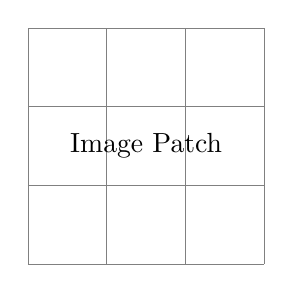
\begin{tikzpicture}[scale=1.0]
      % Draw a simple grid to represent an image patch
      \draw[step=1cm,gray,very thin] (0,0) grid (3,3);
      \node at (1.5,1.5) {Image Patch};
    \end{tikzpicture}
  \end{center}
  \begin{itemize}
    \item Illustrates how the kernel moves across the image.
    \item Each overlapping region produces one output pixel.
  \end{itemize}
\end{frame}

\begin{frame}{Experiment: Manual Convolution Implementation}
  \begin{itemize}
    \item Write a function in Python that performs convolution.
    \item Compare your results with OpenCV's \texttt{filter2D} function.
    \item Experiment with different kernels to observe their effects.
  \end{itemize}
\end{frame}

% ------------------------ Section V: Bridging to CNNs ------------------------
\section{Bridging to Convolutional Neural Networks}

\begin{frame}{From Handcrafted to Learned Filters}
  \begin{itemize}
    \item Traditional methods use manually designed filters.
    \item CNNs automatically learn optimal filters from data.
  \end{itemize}
  \begin{center}
    \includegraphics[width=0.7\textwidth]{cnn_architecture_placeholder.png} % Replace with a diagram of a basic CNN
  \end{center}
\end{frame}

\begin{frame}{Basic CNN Architecture}
  \begin{itemize}
    \item \textbf{Convolutional Layers:} Learn feature detectors.
    \item \textbf{Activation Functions:} Introduce non-linearity.
    \item \textbf{Pooling Layers:} Downsample the feature maps.
    \item \textbf{Fully Connected Layers:} Final classification or regression.
  \end{itemize}
\end{frame}

\begin{frame}{Comparison: Manual vs. Learned Filters}
  \begin{columns}
    \column{0.5\textwidth}
      \textbf{Manual Filters}
      \begin{itemize}
        \item Designed by experts.
        \item Fixed functionality.
      \end{itemize}
    \column{0.5\textwidth}
      \textbf{Learned Filters}
      \begin{itemize}
        \item Learned from data.
        \item Adapt to specific tasks.
      \end{itemize}
  \end{columns}
\end{frame}

\begin{frame}{Optional Notebook Demo: CNN Feature Maps}
  \begin{itemize}
    \item Load a pre-trained CNN model (e.g., on MNIST or CIFAR-10).
    \item Visualize early layer feature maps to connect with manual convolution.
  \end{itemize}
\end{frame}

% ------------------------ Section VI: Wrap-Up ------------------------
\section{Wrap-Up \& Discussion}

\begin{frame}{Summary \& Key Takeaways}
  \begin{itemize}
    \item Traditional image processing laid the groundwork for modern computer vision.
    \item Convolution is the central operation in both traditional filters and CNNs.
    \item CNNs learn to extract features automatically, bridging theory with data-driven methods.
  \end{itemize}
\end{frame}

\begin{frame}{Q \& A / Discussion}
  \begin{center}
    \Huge Questions?
  \end{center}
  \begin{itemize}
    \item What are the limitations of manual filter design?
    \item How does learned filtering in CNNs overcome these limitations?
  \end{itemize}
\end{frame}

\begin{frame}{Future Directions}
  \begin{itemize}
    \item Deeper dive into CNN training and optimization.
    \item Explore advanced computer vision applications.
    \item Hands-on projects using modern deep learning frameworks.
  \end{itemize}
\end{frame}

\end{document}